\documentclass[journal,12pt,twocolumn]{IEEEtran}
%
\usepackage{setspace}
\usepackage{gensymb}
%\doublespacing
\singlespacing

\usepackage{graphicx}
\usepackage[cmex10]{amsmath}
\usepackage{amsmath,amsthm}
\usepackage{mathrsfs}
\usepackage{txfonts}
\usepackage{stfloats}
\usepackage{bm}
\usepackage{cite}
\usepackage{cases}
\usepackage{subfig}

\usepackage{longtable}
\usepackage{multirow}
\usepackage{commath}
\usepackage{enumitem}
\usepackage{mathtools}
\usepackage{steinmetz}
\usepackage{tikz}
\usepackage{circuitikz}
\usepackage{verbatim}
\usepackage{tfrupee}
\usepackage[breaklinks=true]{hyperref}

\usepackage{tkz-euclide}

\usetikzlibrary{calc,math}
\usepackage{listings}
    \usepackage{color}                                            
    \usepackage{array}                                            
    \usepackage{longtable}                                        
    \usepackage{calc}                                             
    \usepackage{multirow}                                         
    \usepackage{hhline}                                           
    \usepackage{ifthen}                                           
    \usepackage{lscape}     
\usepackage{multicol}
\usepackage{chngcntr}

\DeclareMathOperator*{\Res}{Res}

\renewcommand\thesection{\arabic{section}}
\renewcommand\thesubsection{\thesection.\arabic{subsection}}
\renewcommand\thesubsubsection{\thesubsection.\arabic{subsubsection}}

\renewcommand\thesectiondis{\arabic{section}}
\renewcommand\thesubsectiondis{\thesectiondis.\arabic{subsection}}
\renewcommand\thesubsubsectiondis{\thesubsectiondis.\arabic{subsubsection}}

\hyphenation{op-tical net-works semi-conduc-tor}
\def\inputGnumericTable{}                                 

\lstset{
%language=C,
frame=single, 
breaklines=true,
columns=fullflexible
}
\lstset{
%language=TeX,
frame=single, 
breaklines=true
}

\begin{document}

\newtheorem{theorem}{Theorem}[section]
\newtheorem{problem}{Problem}
\newtheorem{proposition}{Proposition}[section]
\newtheorem{lemma}{Lemma}[section]
\newtheorem{corollary}[theorem]{Corollary}
\newtheorem{example}{Example}[section]
\newtheorem{definition}[problem]{Definition}

\newcommand{\BEQA}{\begin{eqnarray}}
\newcommand{\EEQA}{\end{eqnarray}}
\newcommand{\define}{\stackrel{\triangle}{=}}
\bibliographystyle{IEEEtran}
\providecommand{\mbf}{\mathbf}
\providecommand{\pr}[1]{\ensuremath{\Pr\left(#1\right)}}
\providecommand{\qfunc}[1]{\ensuremath{Q\left(#1\right)}}
\providecommand{\sbrak}[1]{\ensuremath{{}\left[#1\right]}}
\providecommand{\lsbrak}[1]{\ensuremath{{}\left[#1\right.}}
\providecommand{\rsbrak}[1]{\ensuremath{{}\left.#1\right]}}
\providecommand{\brak}[1]{\ensuremath{\left(#1\right)}}
\providecommand{\lbrak}[1]{\ensuremath{\left(#1\right.}}
\providecommand{\rbrak}[1]{\ensuremath{\left.#1\right)}}
\providecommand{\cbrak}[1]{\ensuremath{\left\{#1\right\}}}
\providecommand{\lcbrak}[1]{\ensuremath{\left\{#1\right.}}
\providecommand{\rcbrak}[1]{\ensuremath{\left.#1\right\}}}
\theoremstyle{remark}
\newtheorem{rem}{Remark}
\newcommand{\sgn}{\mathop{\mathrm{sgn}}}
\providecommand{\abs}[1]{\(\left\vert#1\right\vert\)}
\providecommand{\res}[1]{\Res\displaylimits_{#1}} 
\providecommand{\norm}[1]{\(\left\lVert#1\right\rVert\)}
%\providecommand{\norm}[1]{\lVert#1\rVert}
\providecommand{\mtx}[1]{\mathbf{#1}}
\providecommand{\mean}[1]{E\(\left[ #1 \right]\)}
\providecommand{\fourier}{\overset{\mathcal{F}}{ \rightleftharpoons}}
%\providecommand{\hilbert}{\overset{\mathcal{H}}{ \rightleftharpoons}}
\providecommand{\system}{\overset{\mathcal{H}}{ \longleftrightarrow}}
	%\newcommand{\solution}[2]{\textbf{Solution:}{#1}}
\newcommand{\solution}{\noindent \textbf{Solution: }}
\newcommand{\cosec}{\,\text{cosec}\,}
\providecommand{\dec}[2]{\ensuremath{\overset{#1}{\underset{#2}{\gtrless}}}}
\newcommand{\myvec}[1]{\ensuremath{\begin{pmatrix}#1\end{pmatrix}}}
\newcommand{\mydet}[1]{\ensuremath{\begin{vmatrix}#1\end{vmatrix}}}
%\numberwithin{equation}{section}
\numberwithin{equation}{subsection}
%\numberwithin{problem}{section}
%\numberwithin{definition}{section}
\makeatletter
\@addtoreset{figure}{problem}
\makeatother
\let\StandardTheFigure\thefigure
\let\vec\mathbf
%\renewcommand{\thefigure}{\theproblem.\arabic{figure}}
\renewcommand{\thefigure}{\theproblem}
%\setlist[enumerate,1]{before=\renewcommand\theequation{\theenumi.\arabic{equation}}
%\counterwithin{equation}{enumi}
%\renewcommand{\theequation}{\arabic{subsection}.\arabic{equation}}
\def\putbox#1#2#3{\makebox[0in][l]{\makebox[#1][l]{}\raisebox{\baselineskip}[0in][0in]{\raisebox{#2}[0in][0in]{#3}}}}
     \def\rightbox#1{\makebox[0in][r]{#1}}
     \def\centbox#1{\makebox[0in]{#1}}
     \def\topbox#1{\raisebox{-\baselineskip}[0in][0in]{#1}}
     \def\midbox#1{\raisebox{-0.5\baselineskip}[0in][0in]{#1}}
\vspace{3cm}
\title{Assignment 2}
\author{Vishal Ashok}
\maketitle
\newpage
%\tableofcontents
\bigskip
\renewcommand{\thefigure}{\theenumi}
\renewcommand{\thetable}{\theenumi}
\begin{abstract}
This document explains how to find the point of intersection of a line and a plane.
\end{abstract}
Download Python code from 
%
\begin{lstlisting}
https://github.com/vishalashok98/AI5106/tree/main/Assignment_1
\end{lstlisting}
%
Download the latex-tikz codes from 
%
\begin{lstlisting}
https://github.com/vishalashok98/AI5106/tree/main/Assignment_1
\end{lstlisting}
%

\section{Problem}
Find the equations of tangents to the circle 
\begin{align}
\vec{x}^T\vec{x}-\myvec{4 & 3}\vec{x}+5 = 0 \label{given_circle_eq}
\end{align}
that are parallel to the line
\begin{align}
\myvec{1 &1}\vec{x}=0 \label{given_line_eq}
\end{align}





	
	



\section{Explanation}
The vector equation of a line can be expressed as 
\begin{align}
    \vec{x} = \vec{q} +\mu\vec{m} \label{vec_eqn_of_line}
\end{align}
The general equation of a second degree can be expressed as :
\begin{align}
\vec{x}^T\vec{V}\vec{x}+2\vec{u}^T\vec{x}+f=0\label{gen__quad_eqn}
\end{align}

\section{Solution}

Comparing \eqref{given_circle_eq} with \eqref{gen__quad_eqn}
\begin{align}
\vec{u}=\myvec{-2 \\ \frac{-3}{2}}, f=5
\end{align}
If $\vec{n}$ is the normal vector of a line, equation of that line can be written as 
\begin{align}
\vec{n}^T\vec{x} = c \label{eq1}
\end{align}
Comparing \eqref{given_line_eq} with \eqref{eq1}
\begin{align}
\vec{n} = \myvec{1 \\ 1}\label{eq2}
\end{align}
Since it is mentioned that the tangent is parallel to given line it will have same normal vector. \\
 The point of contact $\vec{q}$, of a line with a normal vector $\vec{n}$ to the conic in \eqref{gen__quad_eqn} is given by:
\begin{align}
\vec{q} = \vec{V}^{-1}\brak{\kappa \vec{n}-\vec{u}} \label{eq3} \\
\kappa = \pm \sqrt{\frac{\vec{u}^T\vec{V}^{-1}\vec{u}-f}{\vec{n}^T\vec{V}^{-1}\vec{n}}} \label{eq4}
\end{align}
The point of contact $\vec{q}$, of a line with a normal vector $\vec{n}$ to the conic in \eqref{gen__quad_eqn} is given by:
\begin{align}
\vec{q} = \vec{V}^{-1}\brak{\kappa \vec{n}-\vec{u}} \label{eq3} \\
\kappa = \pm \sqrt{\frac{\vec{u}^T\vec{V}^{-1}\vec{u}-f}{\vec{n}^T\vec{V}^{-1}\vec{n}}} \label{eq4}
\end{align}
We know that, for a circle, 
\begin{align}
\vec{V} = \vec{I}  
\end{align}
and from the properties of an Identity matrix, 
\begin{align}
\vec{I}^{-1} &= \vec{I} \\
\vec{I}\vec{X} &= \vec{X}   
\end{align}
Solving for the point of contact using the above equations we get,
\begin{align}
\kappa &= \pm \sqrt{\frac{\myvec{ -2 & -1.5 }\myvec{-2 \\ -1.5} - 5}{\myvec{1 & 1 }\myvec{1 \\ 1 }}} \\
&= \pm \sqrt{\frac{6.25 - 5}{2}} \\
& =  \pm \sqrt{\frac{5}{8}}\\
\end{align}
So there are two tangents to a circle which are parallel to given line which touch circle at two different points  $\vec{q_1}$ and $\vec{q_2}$
\begin{align}
\vec{q_1} &= \myvec{\sqrt{\frac{5}{8}} \\ \sqrt{\frac{5}{8}}} + \myvec{2 \\ \frac{3}{2}} \\
&= \myvec{\frac{279}{100} \\ \frac{229}{100}}
\end{align}
\begin{align}
\vec{q_2} &= \myvec{-\sqrt{\frac{5}{8}} \\ \sqrt{\frac{5}{8}}} + \myvec{2 \\ \frac{3}{2}} \\
&= \myvec{\frac{121}{100} \\ \frac{71}{100}}
\end{align}
Since points $\vec{q_1}$ and $\vec{q_2}$ lie on tangent they satisfy the line equation of tangents, there are two different tangents with same normal vector
\begin{align}
\vec{n}^T\vec{q_1} = c_1 \label{eq1}
\end{align}
\begin{align}
\vec{n}^T\vec{q_2} = c_2 \label{eq1}
\end{align}
$c_1$ and $c_2$ are some constants
\begin{align}
c_1=\myvec{1 & 1}\myvec{\frac{279}{100} \\ \frac{229}{100}}\newline
&= \frac{127}{25}
\end{align}
\newline
\begin{align}
c_2=\myvec{\frac{121}{100} \\ \frac{71}{100}}\newline
&= \frac{48}{25}
\end{align}
So line equations of tangents to the given circle which are parallel to line are
\begin{align}
\myvec{1 &1}\vec{x}=\frac{127}{25}
\end{align}and
\newline
\begin{align}
\myvec{1 &1}\vec{x}=\frac{48}{25}
\end{align}
\newline
\newline
\newline
\newline
\newline
\newline
\newline\newline
\newline
\newline

\begin{figure}[]
\centering
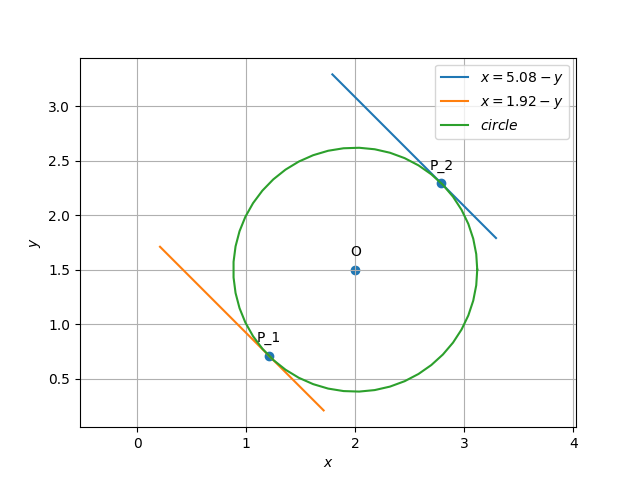
\includegraphics[width=\columnwidth]{Figure_1.png}
\caption{Circle with center (2 1.5) and having the lines (1 1)x =5.08 and (1 1)x =1.92 as tangents with (2.79 2.29) and (1.21 0.71) as point of contact.}
\label{Fig:Circle}
\end{figure}

\end{document}
